\section{Hardware Side - Delivery Infrastructure}
\label{chp:hardware_side}

YouTube was released in 2005 and had an immediate success, resulting in a stunning growth ever since. This growth led to changes in the infrastructure, so that is today more flexible and scalable. In late 2007 Google acquired YouTube and the delivery architecture that initially used third party content distribution network services is now fully operated and managed by Google.
\\
\\
Describing a system like YouTube that constantly evolves is not easy, but a lot of the underlying design principles will most likely stay the same for some time.

\subsection{Steps of downloading a YouTube Video}

Watching a video on YouTube includes downloading the video (or parts of the video) to a client. This downloading process involves different sets of servers, which are necessary for load balancing. The high level steps of accessing a YouTube video are shown in Figure~\vref{fig:video_retrieval}:

\begin{figure}[htbp]
  \begin{center}
    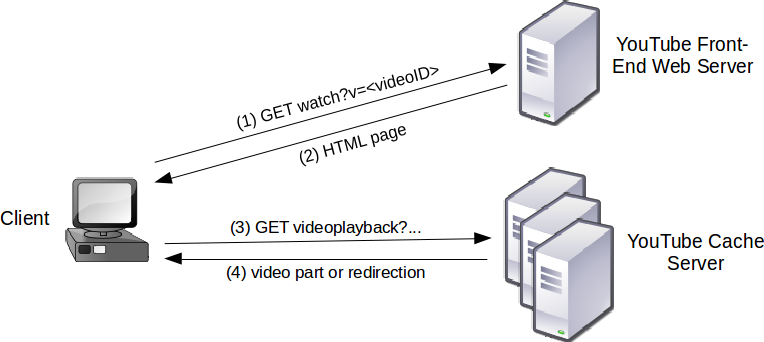
\includegraphics[width=\textwidth]{pictures/video_retrieval.png}
    \caption{High level sequence of steps to retrieve a YouTube video}
    \label{fig:video_retrieval}
  \end{center}
\end{figure}

\begin{enumerate}
  \item The client requests a specific video on the YouTube web page via http://www.youtube.com/watch?v=<videoID>. YouTube has multiple front-end servers for client requests, whereby one server will be responsible for a single request (without considering server crashes).
  
  \item The client downloads the corresponding HTML page. Depending on the video and the profile configuration, the actual video is either embedded through a Adobe Flash Player plugin or a HTML5 video container\footnote{YouTube currently tries to use the HTML5 player always when possible\cite{misc:youtube_html5}}. The relevant container takes further care of the download and the playback of the video. The name of the cache server that will provide the video is among the parameters provided for the plugin or the HTML5 container \cite{inpr:server_selection}.
  
  \item The respective cache server will be queried for the first video part via: \seqsplit{https://<hostname>.googlevideo.com/videoplayback?<request-parameter>}. 

  \item If the cache server has the video and is not overloaded, the server will send the first part of the video ot the client. The client on the other hand will send requests for further video parts, if he keeps watching the respective video part. \\
\\
If the cache server does not have the video or is overloaded, the server will send a redirect message (HTTP 302) to the client indicating another cache server. The request process continues at step 3 again. Thus it is possible, that multiple cache servers are included in the request process.
\end{enumerate}

\subsection{Cache Server Infrastructure}

The cache servers themselves are organized as cache clusters, whereby the servers of one cluster are co-located \cite{inc:video_delivery}. The number of machines per cache cluster is highly variable and depends, among others, on the demand for service issued in the region where the cluster is located and also on the available physical space to host the cache nodes. Each cache node as of 2011 already had a 10 GB / sec network access and 78 TB of disk storage \cite{misc:mmsys_keynote}.
\\
\\
YouTube's cache selection is quite sophisticated and tries to satisfy users by selecting a nearby cache cluster and perform internal redirection to another cache cluster to perform load balancing among cache clusters. The choice of a close-by cache cluster (in terms of RTT) is typically done through DNS resolution. %Each video ID can be deterministically mapped via consistent hashing onto a unique logical name in the lscache namespace, which makes it easy to decide for each cache what portion of the videos it is responsible to serve.
DNS is used for coarse grained load balancing, with a TTL of five minutes. 
\\
\\
The various cache clusters are organized in a three tier hierarchy as shown in Figure~\vref{fig:cache_server}. The global infrastructure of the YouTube caches has been revealed by Adhikari et al. \cite{inpr:vivisecting_youtube} in 2011. They used the distributed infrastructure of the PlanetLab network to request thousands of videos from different vantage points in the world, which allowed to reverse engineer the cache infrastructure and the cache selection policies. 

\begin{figure}[htbp]
  \begin{center}
    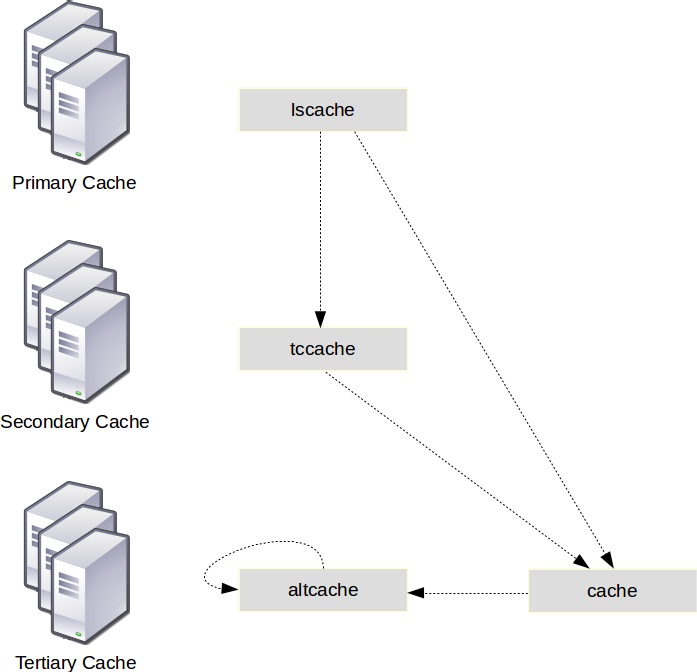
\includegraphics[width=0.9\textwidth]{pictures/cache_server.png}
    \caption{YouTube Cache organization; dashed lines indicate possible redirections}
    \label{fig:cache_server}
  \end{center}
\end{figure}

The three tier caching infrastructure comprises of four different logical namespaces. The machines allocated to the different cache clusters are identified via particular naming conventions. The cache redirection mechanism with these clusters works as follows:

\begin{description}
  \item[Cache Hit] If the video is hot and there are copies at the primary caches, then a logical cache node (lscache namespace) in the primary cache is chosen. If there is no redirection, a machine from a cache cluster serves the video. If the primary cache cluster selected is overloaded, a redirection to a secondary cache cluster (tccache namespace) occurs. The secondary cache can serve the video or redirect it to a tertiary cache site (cache namespace) for load-balancing purposes. Again, in the tertiary cache cluster, the cache server can deliver the video, or perform another redirection. A redirection from a tertiary cache site will remain inside the tertiary cache level and ocur towards a cluster from the altcache namespace. A machine in this namespace now serves the video or redirects it inside the same namespace in case of overload. Very rarely, several redirections occur inside the altcache namespace, with the total number of redirections being limited to 9. For further details
see.

  \item[Cache Miss] If the video is cold and there are no copies at the primary caches, then the request will be most likely redirected from the first level cache to a third level cache. The third level cache will fetch the video from the backend data server, cache it, and deliver the video to the client. It is quite common, as we will see in the next section, that users do not watch the entire video. Therefore, all videos are broken into chunks (of 2 MBytes) and the cache will continue to retrieve from the backend servers new chunks of a video as long as the user keeps viewing that video. Note that despite all the efforts of the engineering team of Google, the cache miss rate remains steadily at about 10\%.
\end{description}

Using traces from a European ISP, Torres et al. [12] observed that as the total number of requests kept increasing, the percentage of requests handled by the closest cache cluster located inside that ISP decreased from 80\% to about 30\%. In this case, DNS request resolution will direct clients to more distant but less loaded cache clusters.\\
The redirections have an impact of the Performance. Each redirection involves:

\begin{enumerate}
  \item DNS query to resolve the hostname of the next cache node,
  \item Opening of a new TCP connection,
  \item Issuing a new video query.
\end{enumerate}

In case of redirections, the final cache server serving the video will most likely not be the closest one in terms of RTT, which has been observed in [12] for the most popular videos of the day. The impact of redirection on the time until the first MByte is downloaded (referred to as video initialization time) has also been studied in [7]. The video initialization time is on average 33\% higher if the video has been fetched through redirections. The fraction of sessions that have been redirected is evaluated in [10]: between 10\% and 30\% of all sessions are redirected at least once. The impact of redirections on the startup delay can also be important [10]:

\begin{itemize}
  \item Without redirections, delays are in the order of milliseconds
  \item With redirections, delay can increase by orders of magnitude, up to 10 seconds
\end{itemize}
